% Options for packages loaded elsewhere
\PassOptionsToPackage{unicode}{hyperref}
\PassOptionsToPackage{hyphens}{url}
%
\documentclass[
  letterpaper,
]{book}

\usepackage{amsmath,amssymb}
\usepackage{iftex}
\ifPDFTeX
  \usepackage[T1]{fontenc}
  \usepackage[utf8]{inputenc}
  \usepackage{textcomp} % provide euro and other symbols
\else % if luatex or xetex
  \usepackage{unicode-math}
  \defaultfontfeatures{Scale=MatchLowercase}
  \defaultfontfeatures[\rmfamily]{Ligatures=TeX,Scale=1}
\fi
\usepackage{lmodern}
\ifPDFTeX\else  
    % xetex/luatex font selection
\fi
% Use upquote if available, for straight quotes in verbatim environments
\IfFileExists{upquote.sty}{\usepackage{upquote}}{}
\IfFileExists{microtype.sty}{% use microtype if available
  \usepackage[]{microtype}
  \UseMicrotypeSet[protrusion]{basicmath} % disable protrusion for tt fonts
}{}
\makeatletter
\@ifundefined{KOMAClassName}{% if non-KOMA class
  \IfFileExists{parskip.sty}{%
    \usepackage{parskip}
  }{% else
    \setlength{\parindent}{0pt}
    \setlength{\parskip}{6pt plus 2pt minus 1pt}}
}{% if KOMA class
  \KOMAoptions{parskip=half}}
\makeatother
\usepackage{xcolor}
\setlength{\emergencystretch}{3em} % prevent overfull lines
\setcounter{secnumdepth}{5}
% Make \paragraph and \subparagraph free-standing
\makeatletter
\ifx\paragraph\undefined\else
  \let\oldparagraph\paragraph
  \renewcommand{\paragraph}{
    \@ifstar
      \xxxParagraphStar
      \xxxParagraphNoStar
  }
  \newcommand{\xxxParagraphStar}[1]{\oldparagraph*{#1}\mbox{}}
  \newcommand{\xxxParagraphNoStar}[1]{\oldparagraph{#1}\mbox{}}
\fi
\ifx\subparagraph\undefined\else
  \let\oldsubparagraph\subparagraph
  \renewcommand{\subparagraph}{
    \@ifstar
      \xxxSubParagraphStar
      \xxxSubParagraphNoStar
  }
  \newcommand{\xxxSubParagraphStar}[1]{\oldsubparagraph*{#1}\mbox{}}
  \newcommand{\xxxSubParagraphNoStar}[1]{\oldsubparagraph{#1}\mbox{}}
\fi
\makeatother


\providecommand{\tightlist}{%
  \setlength{\itemsep}{0pt}\setlength{\parskip}{0pt}}\usepackage{longtable,booktabs,array}
\usepackage{calc} % for calculating minipage widths
% Correct order of tables after \paragraph or \subparagraph
\usepackage{etoolbox}
\makeatletter
\patchcmd\longtable{\par}{\if@noskipsec\mbox{}\fi\par}{}{}
\makeatother
% Allow footnotes in longtable head/foot
\IfFileExists{footnotehyper.sty}{\usepackage{footnotehyper}}{\usepackage{footnote}}
\makesavenoteenv{longtable}
\usepackage{graphicx}
\makeatletter
\newsavebox\pandoc@box
\newcommand*\pandocbounded[1]{% scales image to fit in text height/width
  \sbox\pandoc@box{#1}%
  \Gscale@div\@tempa{\textheight}{\dimexpr\ht\pandoc@box+\dp\pandoc@box\relax}%
  \Gscale@div\@tempb{\linewidth}{\wd\pandoc@box}%
  \ifdim\@tempb\p@<\@tempa\p@\let\@tempa\@tempb\fi% select the smaller of both
  \ifdim\@tempa\p@<\p@\scalebox{\@tempa}{\usebox\pandoc@box}%
  \else\usebox{\pandoc@box}%
  \fi%
}
% Set default figure placement to htbp
\def\fps@figure{htbp}
\makeatother
% definitions for citeproc citations
\NewDocumentCommand\citeproctext{}{}
\NewDocumentCommand\citeproc{mm}{%
  \begingroup\def\citeproctext{#2}\cite{#1}\endgroup}
\makeatletter
 % allow citations to break across lines
 \let\@cite@ofmt\@firstofone
 % avoid brackets around text for \cite:
 \def\@biblabel#1{}
 \def\@cite#1#2{{#1\if@tempswa , #2\fi}}
\makeatother
\newlength{\cslhangindent}
\setlength{\cslhangindent}{1.5em}
\newlength{\csllabelwidth}
\setlength{\csllabelwidth}{3em}
\newenvironment{CSLReferences}[2] % #1 hanging-indent, #2 entry-spacing
 {\begin{list}{}{%
  \setlength{\itemindent}{0pt}
  \setlength{\leftmargin}{0pt}
  \setlength{\parsep}{0pt}
  % turn on hanging indent if param 1 is 1
  \ifodd #1
   \setlength{\leftmargin}{\cslhangindent}
   \setlength{\itemindent}{-1\cslhangindent}
  \fi
  % set entry spacing
  \setlength{\itemsep}{#2\baselineskip}}}
 {\end{list}}
\usepackage{calc}
\newcommand{\CSLBlock}[1]{\hfill\break\parbox[t]{\linewidth}{\strut\ignorespaces#1\strut}}
\newcommand{\CSLLeftMargin}[1]{\parbox[t]{\csllabelwidth}{\strut#1\strut}}
\newcommand{\CSLRightInline}[1]{\parbox[t]{\linewidth - \csllabelwidth}{\strut#1\strut}}
\newcommand{\CSLIndent}[1]{\hspace{\cslhangindent}#1}

\makeatletter
\@ifpackageloaded{bookmark}{}{\usepackage{bookmark}}
\makeatother
\makeatletter
\@ifpackageloaded{caption}{}{\usepackage{caption}}
\AtBeginDocument{%
\ifdefined\contentsname
  \renewcommand*\contentsname{Table of contents}
\else
  \newcommand\contentsname{Table of contents}
\fi
\ifdefined\listfigurename
  \renewcommand*\listfigurename{List of Figures}
\else
  \newcommand\listfigurename{List of Figures}
\fi
\ifdefined\listtablename
  \renewcommand*\listtablename{List of Tables}
\else
  \newcommand\listtablename{List of Tables}
\fi
\ifdefined\figurename
  \renewcommand*\figurename{Figure}
\else
  \newcommand\figurename{Figure}
\fi
\ifdefined\tablename
  \renewcommand*\tablename{Table}
\else
  \newcommand\tablename{Table}
\fi
}
\@ifpackageloaded{float}{}{\usepackage{float}}
\floatstyle{ruled}
\@ifundefined{c@chapter}{\newfloat{codelisting}{h}{lop}}{\newfloat{codelisting}{h}{lop}[chapter]}
\floatname{codelisting}{Listing}
\newcommand*\listoflistings{\listof{codelisting}{List of Listings}}
\makeatother
\makeatletter
\makeatother
\makeatletter
\@ifpackageloaded{caption}{}{\usepackage{caption}}
\@ifpackageloaded{subcaption}{}{\usepackage{subcaption}}
\makeatother

\usepackage{bookmark}

\IfFileExists{xurl.sty}{\usepackage{xurl}}{} % add URL line breaks if available
\urlstyle{same} % disable monospaced font for URLs
\hypersetup{
  pdftitle={Estatística Básica: conceitos e aplicações no R},
  pdfauthor={Henrique José de Paula Alves},
  hidelinks,
  pdfcreator={LaTeX via pandoc}}


\title{Estatística Básica: conceitos e aplicações no R}
\author{Henrique José de Paula Alves}
\date{2026-04-15}

\begin{document}
\frontmatter
\maketitle

\renewcommand*\contentsname{Table of contents}
{
\setcounter{tocdepth}{2}
\tableofcontents
}

\mainmatter
\bookmarksetup{startatroot}

\chapter*{O poder dos dados em um mundo
incerto}\label{o-poder-dos-dados-em-um-mundo-incerto}
\addcontentsline{toc}{chapter}{O poder dos dados em um mundo incerto}

\markboth{O poder dos dados em um mundo incerto}{O poder dos dados em um
mundo incerto}

Vivemos em uma era definida pela abundância de informação. A cada
segundo, uma quantidade sem precedentes de dados é gerada, capturando
desde os nossos hábitos de consumo até os movimentos mais sutis do clima
global. No entanto, dados brutos, por si só, são apenas ruído. Para
transformá-los em conhecimento e ação, precisamos de uma ferramenta
fundamental: a \textbf{Estatística}.

Muitas vezes, somos tentados a confiar em nossa intuição ou no famoso
``instinto'' para tomar decisões. No entanto, a ciência moderna e a
economia comportamental já demonstraram os riscos dessa abordagem.
Decisões baseadas puramente no ``sentimento'' podem ser obscurecidas por
preconceitos e experiências limitadas. A estatística surge como o
antídoto para esse subjetivismo, oferecendo uma estrutura lógica e
rigorosa para separar fatos de suposições.

A importância da estatística transcende as salas de aula e os
laboratórios de pesquisa. Ela é a espinha dorsal da tomada de decisão
baseada em evidências em praticamente todos os setores da sociedade:

\begin{itemize}
\item
  \textbf{Na Saúde:} É através dela que novos tratamentos são testados e
  padrões de doenças são identificados para salvar vidas.
\item
  \textbf{Nos Negócios:} Permite que empresas compreendam tendências de
  mercado e otimizem cadeias de suprimentos, substituindo o palpite pela
  estratégia baseada em números.
\item
  \textbf{No Governo e Sociedade:} Orienta a criação de políticas
  públicas eficazes, desde o planejamento urbano até a resposta a crises
  econômicas.
\item
  \textbf{No Esporte:} Como demonstrado pela famosa revolução do
  \emph{Moneyball}, a análise de dados transformou a maneira como
  equipes são montadas e como o desempenho é avaliado.
\end{itemize}

Este livro convida você a explorar a estatística não apenas como uma
disciplina matemática, mas como uma linguagem universal para entender o
mundo. Ao longo destas páginas, veremos como os métodos estatísticos
funcionam como uma rede de segurança, fornecendo a confiança necessária
para navegar pela incerteza e para fazer escolhas que impactam o
presente e moldam o futuro.

Seja você um estudante, um profissional ou um curioso sobre como o mundo
funciona, compreender a estatística é adquirir a habilidade de enxergar
padrões onde outros veem apenas caos. Bem-vindo à ciência que transforma
dados em inteligência.

\bookmarksetup{startatroot}

\chapter*{Prefácio}\label{prefuxe1cio}
\addcontentsline{toc}{chapter}{Prefácio}

\markboth{Prefácio}{Prefácio}

\textsc{``Lies, damned lies, and statistics''. (Mark Twain, 1891)}

A famosa frase atribuída a Mark Twain resume o medo que muitas pessoas
têm desta disciplina. Este livro foi escrito para provar que a
estatística não é um bicho de sete cabeças, mas sim um superpoder para
entender o mundo.

Escrevi este texto pensando no pesquisador de humanas, no gestor de
marketing e no curioso que deseja entender as notícias sobre pesquisas
eleitorais ou eficácia de medicamentos. Aqui, as equações são mantidas
ao mínimo necessário. Em vez de decorar fórmulas, vamos focar em como
não ser enganado por gráficos tendenciosos e como entender o que a
variabilidade realmente significa.

A estatística é, antes de tudo, a arte de aprender com a experiência.
Vamos começar?

\part{Capítulos}

\chapter{Conceitos básicos}\label{conceitos-buxe1sicos}

\section{Introdução}\label{sec-intro}

Neste capítulo inicial, estabeleceremos as bases fundamentais da
estatística, diferenciando a análise puramente descritiva da inferência,
e definindo os tipos de dados com os quais trabalharemos ao longo deste
livro.

\subsection{O que é Estatística?}\label{o-que-uxe9-estatuxedstica}

A Estatística pode ser definida como a ciência que utiliza a
probabilidade para lidar com a incerteza. Em um mundo inundado por
dados, ela fornece as ferramentas para transformar observações brutas em
conhecimento científico e suporte à decisão.

Podemos dividir a estatística em três grandes pilares:

\begin{enumerate}
\def\labelenumi{\arabic{enumi}.}
\item
  \textbf{Descritiva:} Resume e organiza os dados históricos para
  descrever o que aconteceu, sem tirar conclusões externas
\item
  \textbf{Inferencial:} Usa amostras para tirar conclusões e generalizar
  propriedades sobre uma população inteira sob incerteza.
\item
  \textbf{Preditiva}: utiliza algoritmos estatísticos e técnicas de
  machine learning para definir a probabilidade de eventos futuros com
  base em padrões encontrados em dados do passado.
\end{enumerate}

De modo geral, a Estatística engloba ferramentas teóricas e práticas
visando entender ou analisar o comportamento de informações
quantitativas e/ou qualitativas, medindo incertezas e, dessa forma,
auxiliando na tomada de decisão.

\subsection{Conceitos Fundamentais}\label{conceitos-fundamentais}

Antes de avançarmos para os cálculos, precisamos definir os objetos de
estudo:

\begin{itemize}
\item
  \textbf{População:} O conjunto total de elementos que compartilham
  pelo menos uma característica comum (ex: todos os domicílios do
  Brasil).
\item
  \textbf{Parâmetro:} Uma medida numérica que descreve uma
  característica da população (geralmente desconhecida e representada
  por letras gregas como \(\mu\), \(\sigma\)).
\item
  \textbf{Amostra:} Um subconjunto representativo da população
  (\(\bar{X}\), \(S\))
\item
  \textbf{Estimativa (ou Estatística):} Uma medida numérica calculada a
  partir de dados amostrais para estimar um parâmetro.
\end{itemize}

\begin{figure}[H]

{\centering 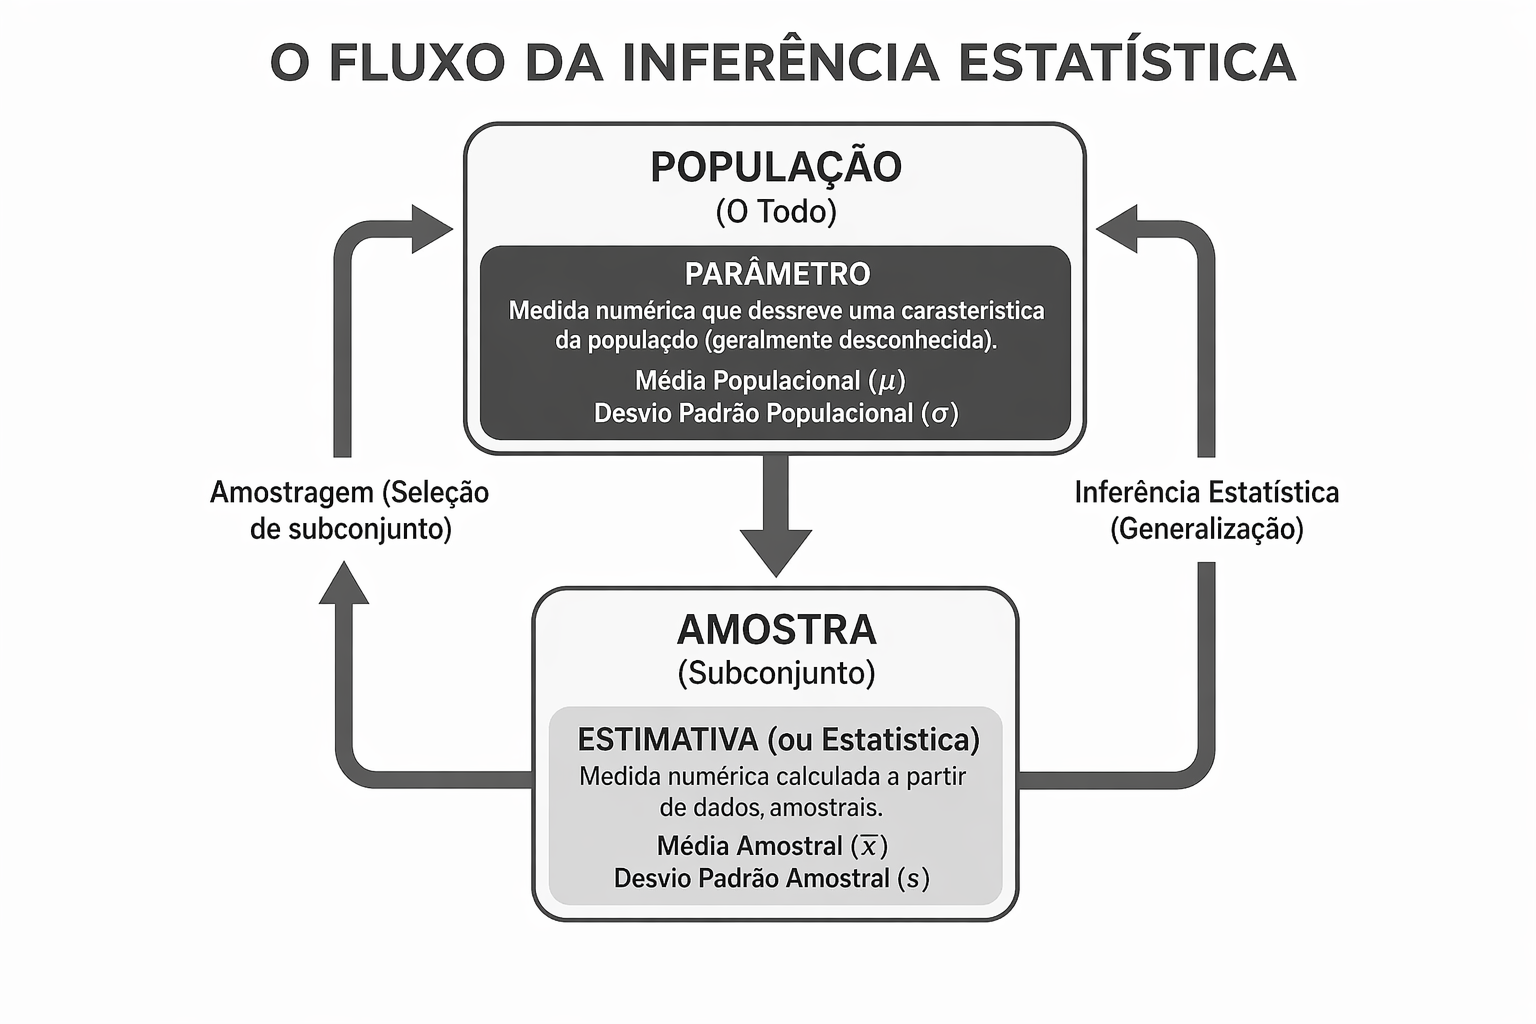
\includegraphics[width=5.71875in,height=\textheight,keepaspectratio]{images/clipboard-3880653047.png}

}

\caption{Figura 1: O Fluxo da Inferência Estatística entre População e
Amostra.}

\end{figure}%

Alguns conceitos e definições matemáticas bem como suas propriedades são
de extrema importância para um bom entendimento das técnicas de análise
estatística. Entretanto, não será apresentado um capítulo a parte sobre
esses conceitos e definições. Ao longo do livro, à medida que for sendo
necessário, estes serão apresentados da forma mais simples possível, sem
o rigor matemático. No próximo capítulo, vamos tratar da análise
exploratória de dados.

\chapter{Análise Exploratória}\label{anuxe1lise-exploratuxf3ria}

\section{Introdução}\label{introduuxe7uxe3o}

Em linhas gerais, a análise exploratória de dados tem ligação direta com
a organização e descrição dos dados, reunindo uma quantidade razoável de
ferramentas e recursos que auxiliam na interpretação dos valores
observados ou amostrados. Exemplificando sua utilidade, a avaliação de
como as observações se distribuem, bem como onde estão posicionadas e,
ainda, como se apresentam em termos de dispersão e associação.

Neste capítulo, será introduzido conceitos e métodos de exploração de
dados, um passo fundamental para análises estatísticas completas e
avançadas.

\subsection{Variáveis}\label{variuxe1veis}

Em linhas gerais, trata-se de uma característica medida na população ou
na amostra. Como exemplos, apresentam-se a altura de um indivíduo, o
peso, a temperatura, a cor dos olhos, o número de filhos, a cor das
folhas de uma planta, entre outros. São representadas por letras
maiúsculas do nosso alfabeto: X, Y, A, B, W.

A Figura 2 apresenta um esquema de classificação das variáveis.

\begin{figure}[H]

{\centering 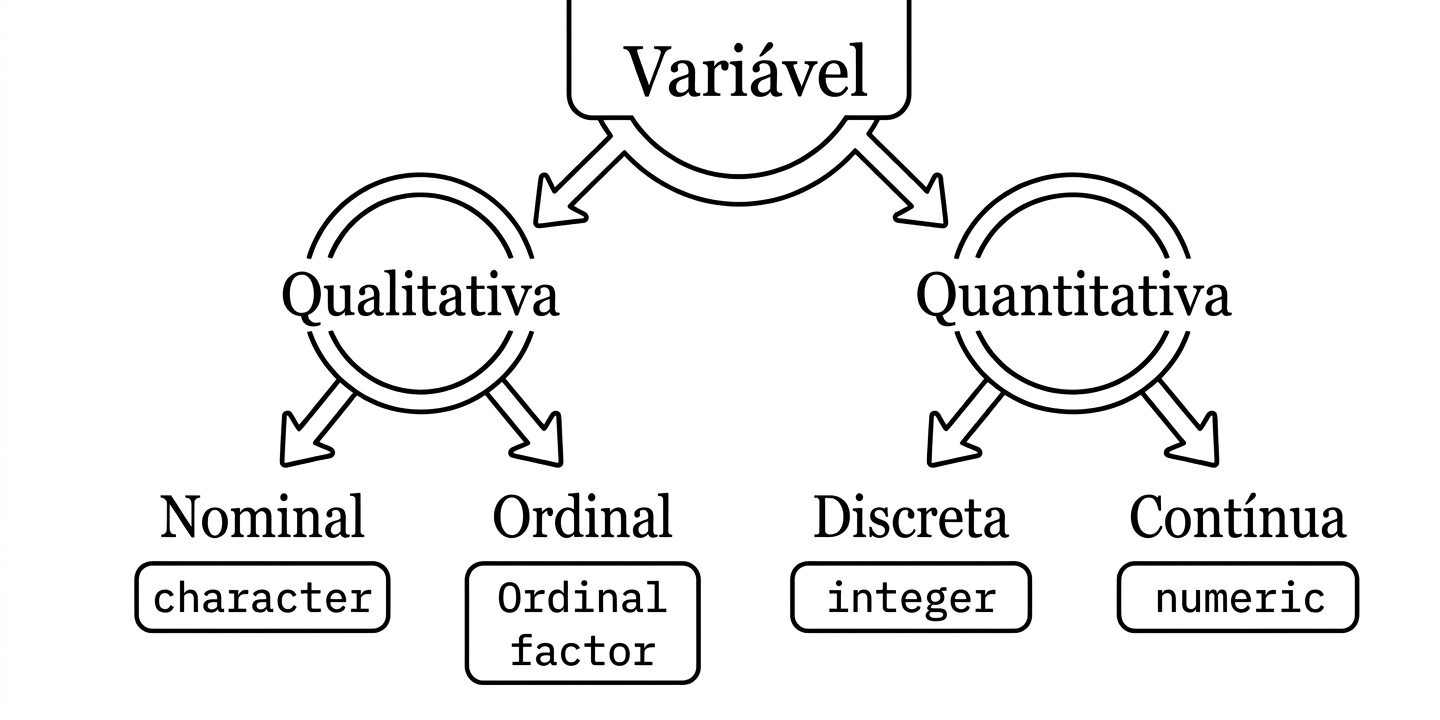
\includegraphics[width=5.71875in,height=\textheight,keepaspectratio]{images/fig3.png}

}

\caption{Figura 2: Esquema de classificação de variáveis.}

\end{figure}%

\subsubsection{Variável Qualitativa
Nominal}\label{variuxe1vel-qualitativa-nominal}

As variáveis qualitativas nominais apresentam o menor grau de informação
dentre os quatro tipos apresentados. É possível apenas a avaliação de
frequências e ordenações arbitrárias. O sexo, a religião, a raça, a cor
preferida, são exemplos desse tipo de variável

Exemplo: Sexo de uma pessoa

Suponha uma pesquisa com aplicação de um questionário on-line, onde o
sexo dos entrevistados é perguntado. Suponha ainda que a variável
\emph{Sexo de uma pessoa} seja representada por X, as observações podem
ser:

X:\{Masculino, Masculino, Feminino, Masculino, Feminino, Feminino,
\ldots, Feminino\}

\part{final.qmd}

\chapter{Considerações finais}\label{considerauxe7uxf5es-finais}

\chapter*{References}\label{references}
\addcontentsline{toc}{chapter}{References}

\markboth{References}{References}

\phantomsection\label{refs}
\begin{CSLReferences}{0}{1}
\end{CSLReferences}


\backmatter


\end{document}
